% This is a basic Math Paper

\documentclass[11pt]{article}

% Preamble

\usepackage[margin=1in]{geometry}
\usepackage{amsfonts, amsmath, amssymb}
\usepackage{fancyhdr, float, graphicx}
\usepackage[utf8]{inputenc} % Required for inputting international characters
\usepackage[T1]{fontenc} % Output font encoding for international characters
\usepackage{fouriernc} % Use the New Century Schoolbook font
\usepackage[nottoc, notlot, notlof]{tocbibind}
\usepackage{url}
\usepackage{placeins}
\usepackage{multirow}
% Header and Footer
\pagestyle{fancy}
\fancyhead{}
\fancyfoot{}
\fancyhead[L]{\textit{\Large{Experiment 1: Newton's Rings}}}
%\fancyhead[R]{\textit{something}}
\fancyfoot[C]{\thepage}
\renewcommand{\footrulewidth}{1pt}



% Other Doc Editing
% \parindent 0ex
%\renewcommand{\baselinestretch}{1.5}

\begin{document}
	
	\begin{titlepage} 
		\centering 
		
		%---------------------------NAMES-------------------------------
		
		\huge\textsc{
			MIT World Peace University
		}\\
	
		\vspace{0.75\baselineskip} % space after Uni Name
		
		\LARGE{
			Physics\\
			First Year B. Tech, Trimester 3\\
			Academic Year 2021-22
		}
		
		\vfill % space after Sub Name
		
		%--------------------------TITLE-------------------------------
		
		\rule{\textwidth}{1.6pt}\vspace*{-\baselineskip}\vspace*{2pt}
		\rule{\textwidth}{0.6pt}
		\vspace{0.75\baselineskip} % Whitespace above the title
		
		
		
		\huge{\textsc{
				Measuring the radius of curvature of a plano-
				convex lens using Newton’s rings apparatus
			}} \\
		
		
		
		\vspace{0.5\baselineskip} % Whitespace below the title
		\rule{\textwidth}{0.6pt}\vspace*{-\baselineskip}\vspace*{2.8pt}
		\rule{\textwidth}{1.6pt}
		
		\vspace{1\baselineskip} % Whitespace after the title block

		%--------------------------SUBTITLE --------------------------	
			
		\LARGE\textsc{
			Experiment No. 1
		} % Subtitle or further description
		\vfill
		
		%--------------------------AUTHOR-------------------------------
		
		Prepared By
		\vspace{0.5\baselineskip} % Whitespace before the editors
		
		\Large{
			109054. Krishnaraj Thadesar
			
			Division 9 Batch I3
		}
		
		
		\vspace{0.5\baselineskip} % Whitespace below the editor list
		\today

	\end{titlepage}

	\begin{center}
	{\Large Pledge}\\
	\vspace{0.5cm}
	I solemnly affirm that I am presenting this journal based on my own experimental work. I have neither copied the observations, calculations, graphs and results from others nor given it to others for copying.\\
		\end{center}
	
	\vspace{0.5cm}
	
    \begin{flushright}
	{\large Signature of the student}\\
	\vspace{1cm}
	 \end{flushright}
	
	
	
	\begin{center}
		{\LARGE Experiment 1: Newton's Rings}\\
	\end{center}

	\section{Aim}
	\noindent
	To measure the radius of curvature of a planoconex lens using Newton's rings apparatus\\
	
	\section{Apparatus}

	\begin{enumerate}
		\item Newton's rings apparatus consisting of
		
		\begin{enumerate}
			\item Planoconvex lens
			\item Optically flat glass plate
			\item Beam splitter
			\item T-type traveling microscope with scale with L.C. $=0.001 \mathrm{~cm}$
		\end{enumerate}
		\item Monochromatic source of light of known wavelength (ex. Sodium)
		\item Reading lamp and reading lens
	\end{enumerate}


	\section{Significance of the Experiment}
	\textit{Newton's rings apparatus can be considered as an interferometer, since it generates a steady state and well defined interference pattern. One of the prime applications of interferometers is precise measurements of dimensions. This experiment aims at a precise measurement of radius of curvature of a plano-convex lens using 'Newton's interferometer'. The other applications of this apparatus are, measuring the wavelength of monochromatic source of light, refractive index of the liquids and testing preciseness of glass plates and lenses.}
	
	
	\section{Theory}
	Newton's rings are the concentric and circular fringes obtained by using interference of circularly symmetric wedge shaped films. (Refer Fig. $1.1$ a, b and c). Such film can be obtained by placing a planoconvex lens on a glass plate. The region between these two components forms a circularly symmetric wedge shaped film, as the locus of points having same path difference forms a circle. If this film is exposed to a plane wavefront of monochromatic light from the top, then the rays reflected from the top and bottom of the circularly symmetric wedge shaped film interfere and produce Newton's rings\\
	
	Thus if diameters of Newton's rings are measured then a few important physical quantities such as $R, \lambda$ and $\mu$ of the liquid can be measured.\\
	
	\begin{figure}[H]
		\centering
		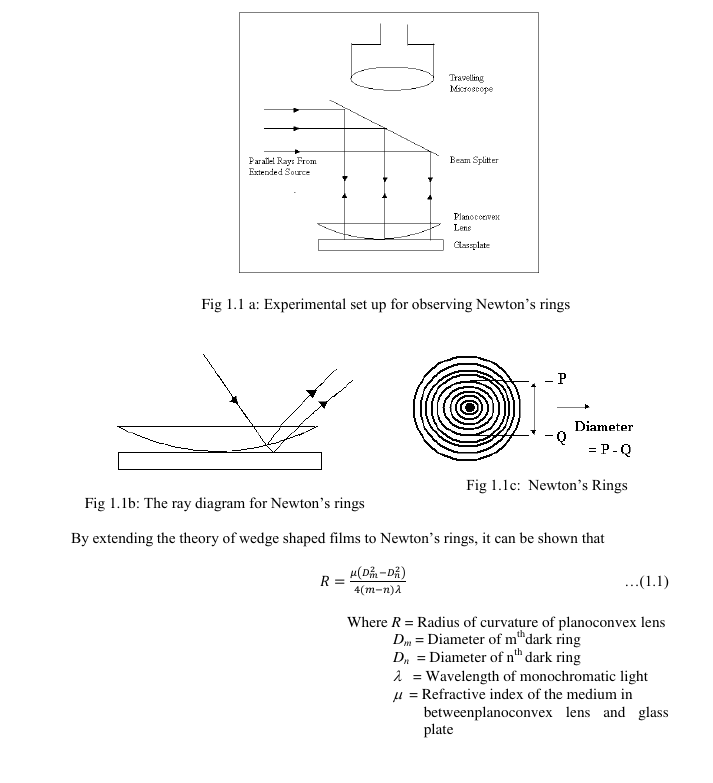
\includegraphics[scale=0.9]{theory.png}
		\label{it}
	\end{figure}
	\clearpage
	
	\section{Procedure}
	
	\begin{enumerate}
		\item Produce Newton's rings by the procedure given below.
		\begin{enumerate}
			\item Make every component dust free.
			\item	Level the whole apparatus using spirit level
			\item Keep the wooden boxes containing a beam splitter and glass plate below the $T$ type microscope. Keep planoconvex lens on the glass plate exactly below the microscope such that its curved part touches the glass plate
			\item Render a parallel wavefront of sodium by placing the source at the focal length of a lens. Expose planoconvex lens-glass plate system parallel wavefront of light. Now Newton's rings can be seen through the microscope.
			\item Adjust the eyepiece of the microscope so that sharp Newton's rings are produced
			\item . If the central ring is not dark then gently tap the apparatus to make the centre dark. The central ring should be dark throughout the experiment.
		\end{enumerate}
	
		\item The central dark ring is the zero ${ }^{\text {th }}$ one. Measure the diameters of first five dark rings by using the procedure given below
		\begin{enumerate}
			\item Move the microscope, so that crosswire is adjusted on upper part of the first dark ring. Measure this position, say $P$ on the scale of the microscope, in the following manner
				$$
				\mathrm{P}=\mathrm{MSR}+\mathrm{VSR} \times \mathrm{LC} \mathrm{cm}
				$$
				Where \textbf{\underline{MSR}} is the reading on main scale which coincides with the zero of the vernier scale. If no reading coincides, then the reading on the main sale previous to with the zero of the vernier
				\textbf{\underline{VSR}} is the sequence number of division on the vernier scale which exactly coincides with the division on the main scale.
				$\underline{\mathbf{L C}}$ is the least  
				count of the scale of the microscope
			\item Move the microscope down to adjust the crosswire on the lower part of first dark ring. Measure the corresponding position on the scale, say, $Q$ by using the procedure given above
			\item The diameter of the ring is $P-Q \mathrm{~cm}$
			\item Repeat the above procedure for measuring the diameters of $2^{\text {nd }}, 3^{\text {rd }}, ^{\text {th }}$ and $5^{\text {th }}$ dark rings
	
\end{enumerate}
	\item Plot the graph of $D_{n}^{2} V s n$. Calculate the slope of this graph. The slope gives the precise value of $\left(\frac{D_{m}^{2}-D_{n}^{2}}{m-n}\right)$
	\item Calculate the radius of curvature of planoconvex lens by using formula (1.1). Take $\mu=1$, as in this experiment, Newton's rings are produced in air. The source used is sodium, therefore take $\lambda=5890 \quad \mathrm{~A}^{\circ}=5890 \times 10^{-8} \mathrm{~cm}$
	\item Compare this $\mathrm{R}_{\mathrm{e}}$ with the standard radius of curvature $\left(\mathrm{R}_{\mathrm{s}}\right)$ given. Calculate the percentage deviation, which needs to be as less as possible.
	\end{enumerate}
\clearpage

	\section{Observations}

	\begin{table}[H]
\centering
\begin{tabular}{|l|l|}
	\hline Smallest Division on the main scale & 0.5 mm \\
	\hline Number of Divisions on vernier scale & 50\\
	\hline L.C. of traveling microscope & 0.001 cm\\
	\hline
\end{tabular}
\caption{Table 1.1: Calculation of the least count of the scale on microscope.}
\end{table}

	\begin{table}[H]
		\centering
		$$
		\begin{array}{|c|c|c|c|c|}
			\hline \begin{array}{c}
				\text { Seq. no. of } \\
				\text { Dark ring } \\
				(n)
			\end{array} & \begin{array}{c}
				\text { Upper } \\
				\text { position } \\
				(P), \boldsymbol{c m}
			\end{array} & \begin{array}{c}
				\text { Lower } \\
				\text { position } \\
				(Q), \boldsymbol{c m}
			\end{array} & \begin{array}{c}
				\text { Diameter } \\
				D_{n} = \boldsymbol{P}-Q \\
				\mathrm{~cm}
			\end{array} & \begin{array}{c}
				\text { Square of } \\
				\text { diameter } \\
				D_{n}^{2}, \mathrm{~cm}^{2}
			\end{array} \\
			\hline 1 & 5.016 & 4.904 & 0.112 & 0.012 \\
			\hline 2 & 4.973 & 4.818 & 0.155 & 0.024\\
			\hline 3 & 4.941 & 4.754 & 0.187 & 0.035\\
			\hline 4 & 4.914 & 4.701 & 0.213 & 0.453\\
			\hline
		\end{array}
		$$
	\caption{Table (1.2) Diameters of Newton's rings}
	\end{table}
	\section{Calculations:}
	
	
	Slope of the graph of $D_{n}^{2} \text{  Vs  } n=$ 0.012$ \mathrm{ cm}^{2}$\\
	Wavelength of sodium source used in the experiment $=5890 \mathrm{~A}^{\circ}$\\
	Radius of curvature of planoconvex lens = \\
	$$
	R_{e}=\frac{\mu\left(D_{m}^{2}-D_{n}^{2}\right)}{4(m-n) \lambda}=\frac{1 \times 0.012}{4 \times \lambda}=\frac{1 \times 0.012}{4 \times 5890 \times 10^{-8}}=\underline{50.9337 \mathrm{ cm}}
	$$

	$$
	\begin{array}{|c|c|c|}
		\hline \begin{array}{c}
			\text { Standard radius of } \\
			\text { curvature } \\
			R_{s}, \mathrm{~cm}
		\end{array} & \begin{array}{c}
			\text { Radius of curvature using } \\
			\text { Newton's rings } \\
			R_{e}, \mathrm{~cm}
		\end{array} & \% \text { deviation }=\left|\frac{R_{s}-R_{e}}{R_{s}}\right| \times 100 \% \\
		\hline 50 cm & 50.9337 & 1.8674  \% \\
		\hline
	\end{array}
	$$

	\clearpage

\section{Graphs}

		\begin{figure}[H]
		\centering
		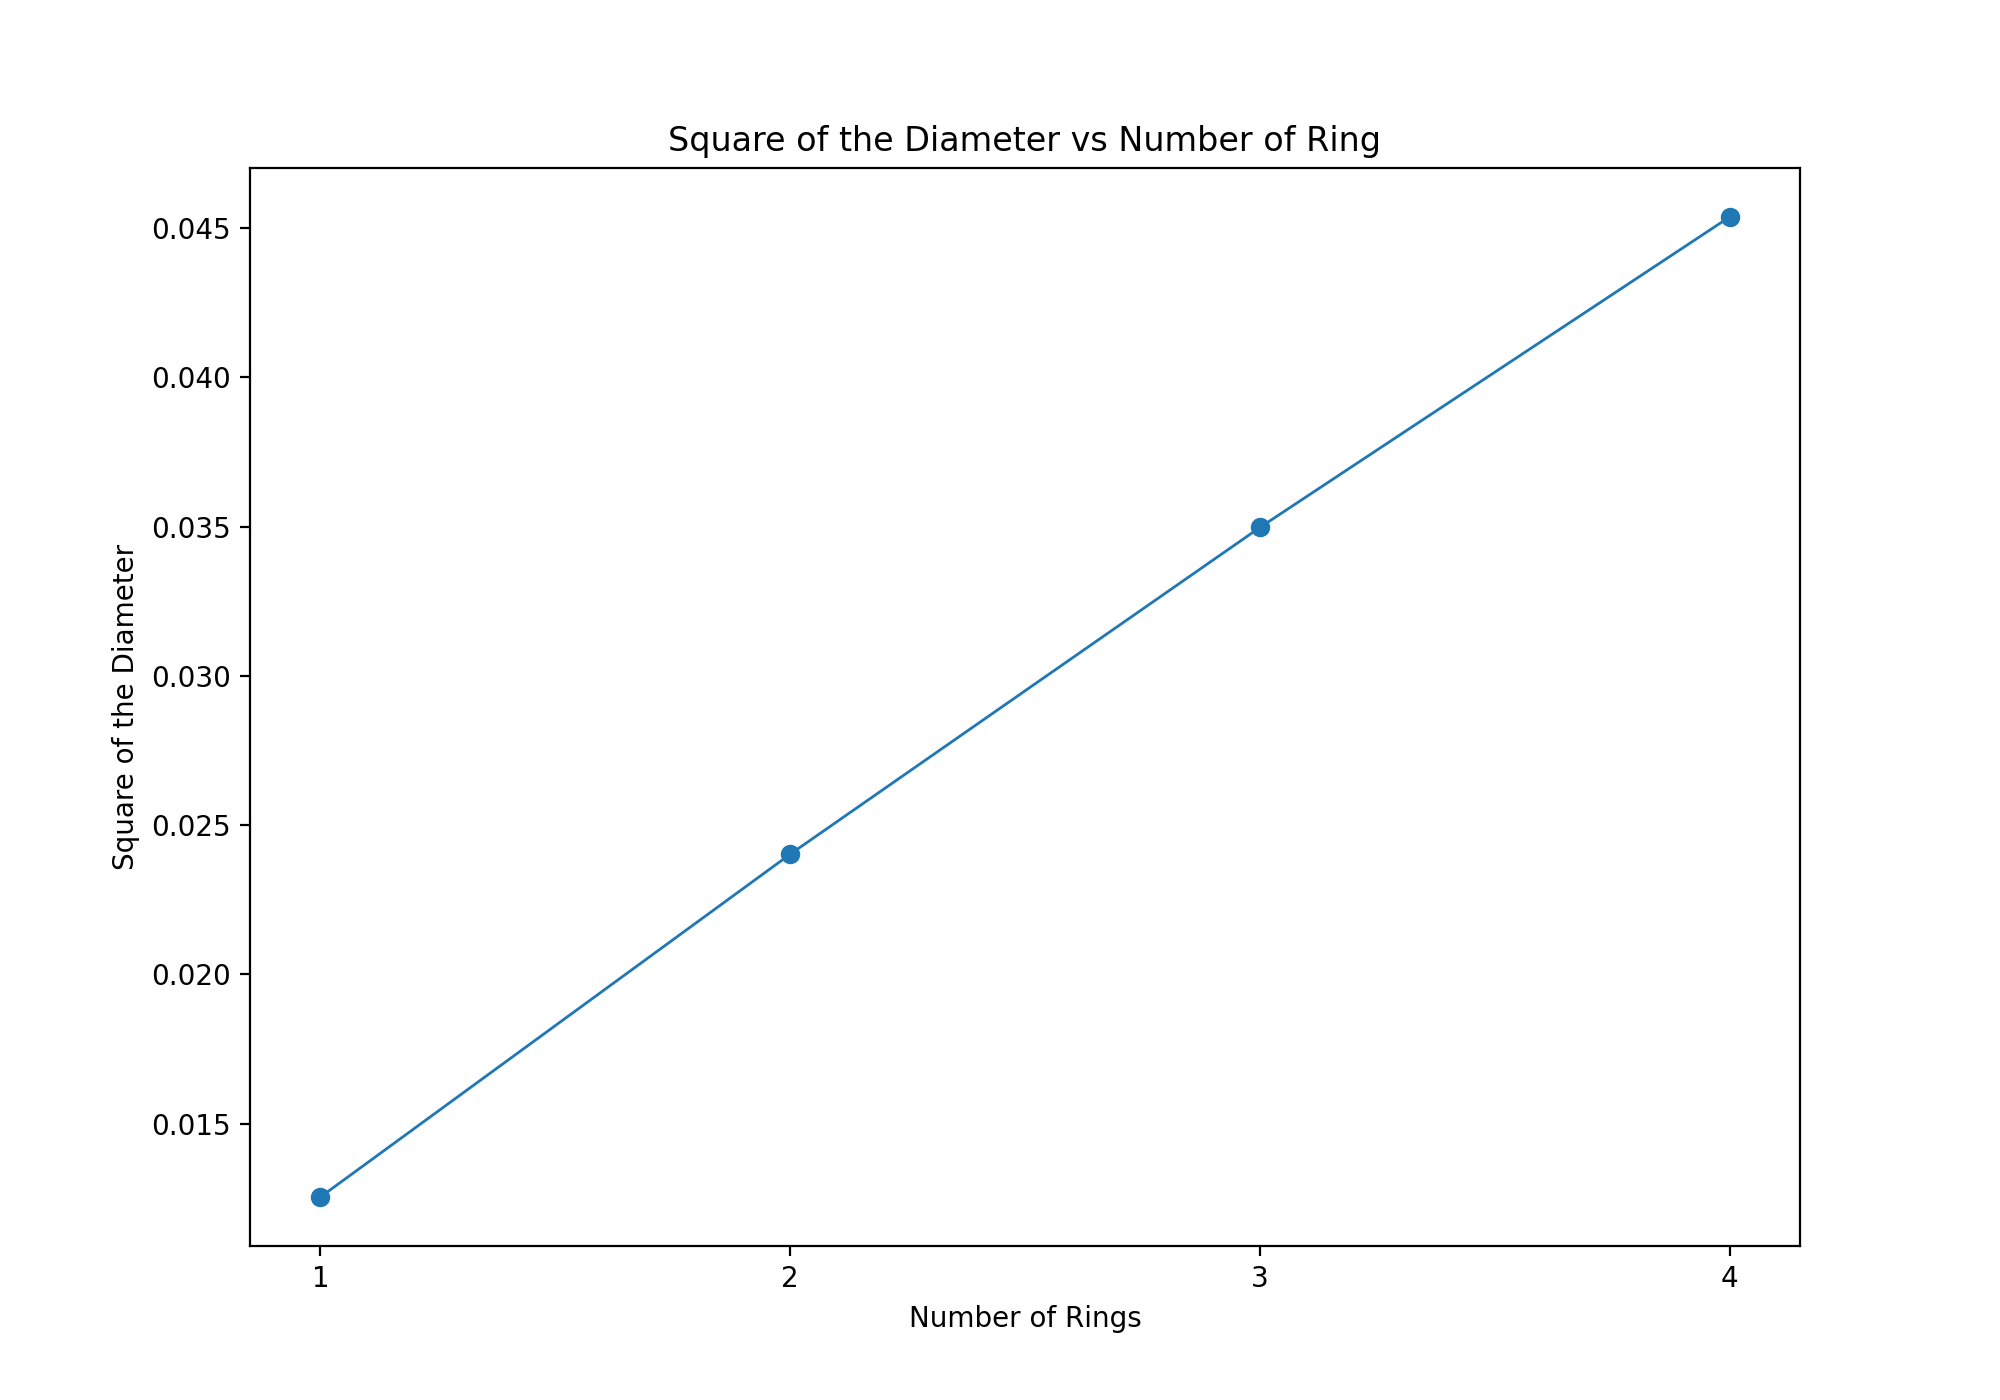
\includegraphics[scale=0.6]{plot.png}
		\label{it}
		\end{figure}
	
	Slope = $$\frac{y_2^2 - y_1^2}{x_2 -x_1} = \frac{D_2^2 - D_1^2}{2 -1} $$
					$$ = \frac{0.024 - 0.012}{2-1} = 0.012 cm^2$$

	\section{My Understanding of the Experiment}
	This experiment was studied deeply by Newtons, and hence gets its name. It's important as supports the wave theory of light by showing decisive and predictable proof of its interference to produce concentric dark and bright circular fringes of light. To interfere, atleast 2 waves of light are needed, which have a difference in their phase. \\	
	
	This phase difference is created in this case, as a plano convex lens is kept over a glass plate. This naturally creates some air gap between them, thereby causing the light to reflect, as well as refract, in such a way that the required phase change is achieved. The better the glass surface is, the better and sharper is the interference pattern. \textit{Because of that, checking the uniformity of a glass surface is one of its major applications. }

\end{document}